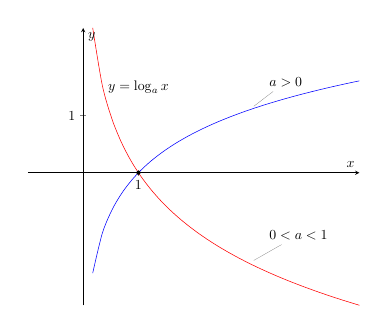
\begin{tikzpicture}[scale=0.5]
\begin{axis}[
 axis lines=middle,
 ticklabel style={fill=white},
xmin=-1.,%xmax=1.5,
%ymin=-1,ymax=5,
 xlabel=$x$,ylabel=$y$,
 domain=0:5,
 samples=30,
 smooth,
 xtick={1},ytick={1},
 yticklabels={1},   xticklabels={1},
 width=10cm]
\coordinate  (x2) at (1,e);
\coordinate  (x1) at (1,0);
\addplot[blue] {ln(x)};
\addplot[red] {(ln(x)/ln(0.5))};
\fill[black] (x2) circle (1.5pt);
\fill[black] (x1) circle (1.5pt);

\node[] at (axis cs:1,{1.5}) {$y=\log_a{x}$};

\node[pin= 50:{$a>0$}] at (axis cs:3,{ln(3)}) {};
\node[pin= 50:{$0<a<1$}] at (axis cs:3,{(ln(3)/ln(0.5)}) {};
\end{axis}
\end{tikzpicture}